\documentclass[Output/slides.tex]{subfiles}
\begin{document}
\section{Incomplete Information}
\begin{frame}{Incomplete Information: Setup}
\begin{itemize}
  \item Nature selects state:
    \begin{itemize}
      \item \(\omega_i\): player \(i\) can commit first, prob.\ \(\mu\).
      \item \(\omega_{-i}\): player \(-i\) can commit first, prob.\ \(\mu\).
      \item \(\omega_\emptyset\): simultaneous commitment, prob.\ \(1-2\mu\).
    \end{itemize}
  \item Importantly, if player $i$ can commit first but decides to wait, player $-i$ has the option to commit second before the base game is played \pause
  \item Players have uncertainty over states, player \(i\) receives signals
    \[
      \sigma_i(\omega_i)=\sigma_i(\omega_\emptyset)=t_\emptyset,\quad
      \sigma_i(\omega_{-i})=t_{-i}.
    \]
  \item Beliefs upon \(t_\emptyset\):
    \[
      P(\omega_i \mid t_\emptyset)=\tfrac{\mu}{1-\mu},\quad
      P(\omega_\emptyset \mid t_\emptyset)=\tfrac{1-2\mu}{1-\mu}.
    \]
\end{itemize}
\end{frame}
\begin{frame}{Incomplete Information: Payoff Functions}
Assume player \(-i\), upon receiving \(t_\emptyset\), randomizes over 
\(\{S_1, M_1, W\}\) with probabilities \(p,\;q,\;1-p-q\).  
Then player \(i\)’s payoff upon receiving \(t_\emptyset\) is:
\pause
\vspace{0.3ex}
\footnotesize
\begin{align*}
U_i\bigl(S_1 \mid t_\emptyset\bigr)
&= P_i(\omega_i\mid t_\emptyset)\cdot 1 \\
&\quad + P_i(\omega_\emptyset\mid t_\emptyset) \cdot \bigl[ p(-1) + q(1) + (1 - p - q)(1) \bigr], \\
\\
U_i\bigl(M_1 \mid t_\emptyset\bigr)
&= P_i(\omega_i\mid t_\emptyset)\cdot (-\tfrac{1}{2}) \\
&\quad + P_i(\omega_\emptyset\mid t_\emptyset) \cdot \bigl[ p(-\tfrac{1}{2}) + q(0) + (1 - p - q)(-\tfrac{1}{2}) \bigr], \\
\\
U_i\bigl(W \mid t_\emptyset\bigr)
&= P_i(\omega_i\mid t_\emptyset)\cdot (-\tfrac{1}{2}) \\
&\quad + P_i(\omega_\emptyset\mid t_\emptyset) \cdot \bigl[ p(-\tfrac{1}{2}) + q(1) + (1 - p - q)(-\tfrac{1}{3}) \bigr].
\end{align*}
\normalsize
\vspace{0.5ex}
\emph{\(M_1\) is weakly dominated by \(W\).}
\end{frame}
\begin{frame}{Incomplete Information: Symmetric Mixed Equilibrium}
\small
When \(\mu \le 0.2\), there is a unique symmetric equilibrium in mixed strategies:
\[
\sigma_i(S_1 \mid t_\emptyset) \;=\; p(\mu)
\;=\;\frac{8 - 7\mu}{11\,(1 - 2\mu)},
\qquad
\sigma_i(W \mid t_\emptyset) \;=\; 1 - p(\mu).
\]
Players never choose \(M_1\). 
\end{frame}
\begin{frame}{Payoff and miscoordination vs.\ \(\mu\)}
\centering
\begin{minipage}{0.48\linewidth}
\centering
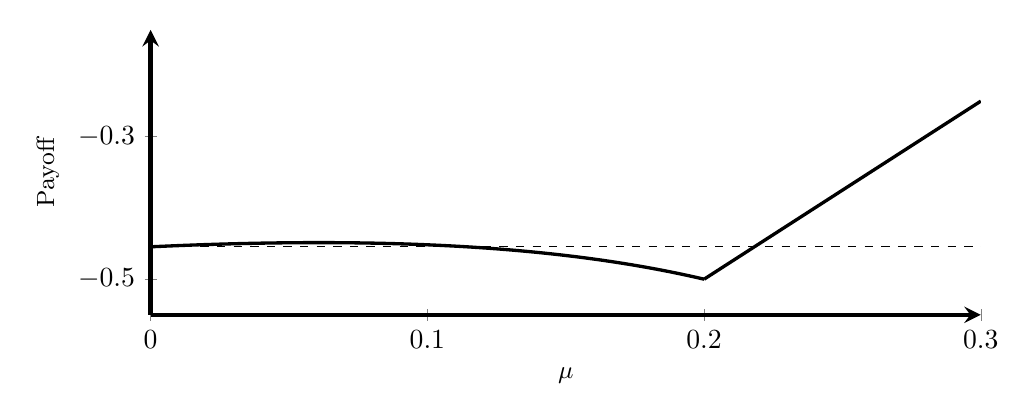
\begin{tikzpicture}
\begin{axis}[width=\linewidth,height=5.2cm,
    xmin=0,xmax=.3,ymin=-.55,ymax=-.15,
    axis x line=bottom, axis y line=left,
    xlabel={\small\(\mu\)}, ylabel={\small Payoff},
    xtick={0,.1,.2,.3},ytick={-0.5,-0.3},
    axis line style={ultra thick}]
  \addplot[very thick,domain=0:0.2,samples=200]
    {(3*x-5)/11 + (-2*x-23*x*x)/(22*(1-2*x))};
  \addplot[very thick,domain=0.2:0.3,samples=200]{2.5*x-1};
  \addplot[dashed] coordinates {(0,-5/11)(0.3,-5/11)};
\end{axis}
\end{tikzpicture}\\[2pt]
\small Equilibrium payoff
\end{minipage}
\hfill
\begin{minipage}{0.48\linewidth}
\centering
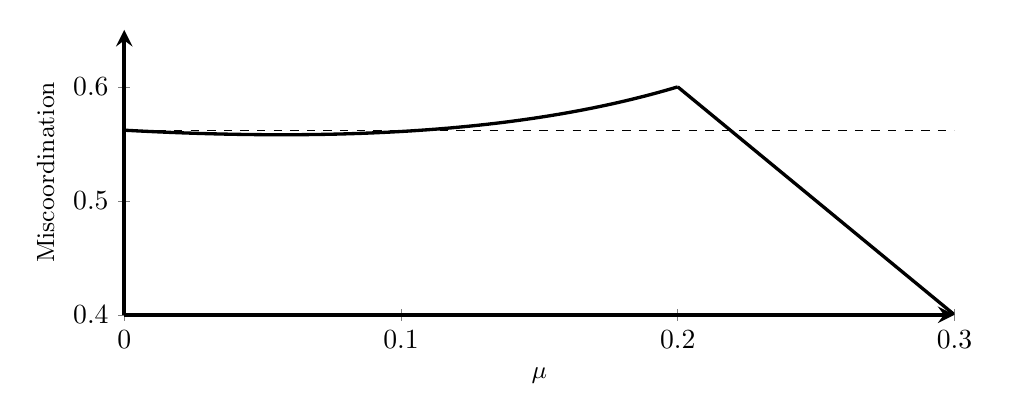
\begin{tikzpicture}
\begin{axis}[width=\linewidth,height=5.2cm,
    xmin=0,xmax=.3,ymin=.4,ymax=.65,
    axis x line=bottom, axis y line=left,
    xlabel={\small\(\mu\)}, ylabel={\small Miscoordination},
    xtick={0,.1,.2,.3},ytick={.4,.5,.6},
    axis line style={ultra thick}]
  \addplot[very thick,domain=0:0.2,samples=250]
    {(149*x*x-152*x+68)/(121*(1-2*x))};
  \addplot[very thick,domain=0.2:0.3,samples=200]{1-2*x};
  \addplot[dashed] coordinates {(0,68/121)(0.3,68/121)};
\end{axis}
\end{tikzpicture}\\[2pt]
\small Probability of miscoordination
\end{minipage}
\end{frame}
\end{document}